\clearpage


%%-- acoustic measurement
\begin{figure}[H]
 \centering
 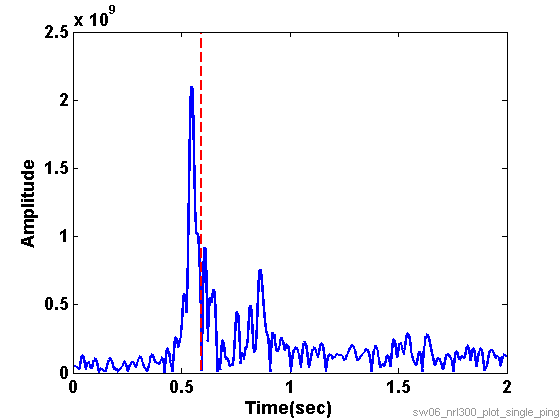
\includegraphics[width=0.5\textwidth]{sw06_nrl300_single_ping.png}
 \caption{Matched filter output of received chirp signal on VLA Shark at GMT 20:30:04, Aug 16th. The red dash line shows the centroid arrival time, which is different than the peak arrival time. }\label{fig:nrl300_single}
\end{figure}
%%--F1
%\begin{figure}[H]
%  \centering
%  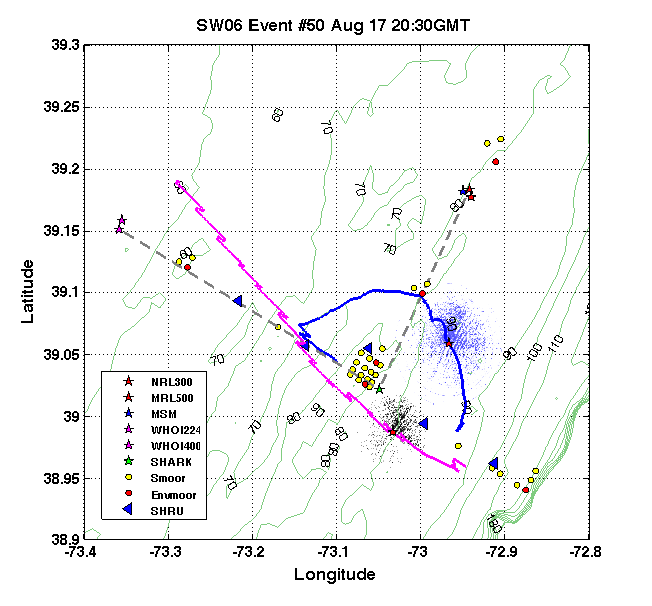
\includegraphics[width=\textwidth]{Aug17_2030_t.png}
%  \caption{Surface expression of internal wave package at 20:30GMT, Aug. 17, recorded by R/V Sharp and R/V Oceanus. Blue and red lines indicate their movements, respectively. (Blue: R/V Sharp's, red: R/V Oceanus'}\label{fig:r2130_r}
%\end{figure}

%
%\begin{figure}[H]
% \centering
% 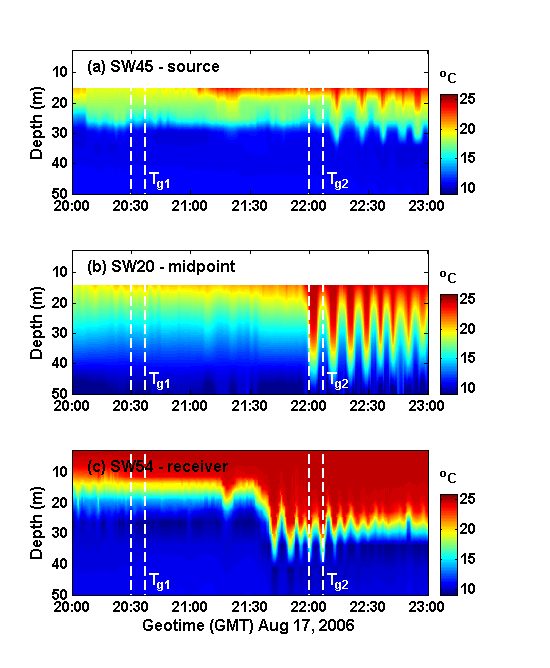
\includegraphics[width=0.5\textwidth]{jasa2_temperature.png}
% \caption{Temperature record at three location along the fixed sourc-receiver track. Panel (a), (b) and (c) show the temperature at the NRL300 source (SW45), the midpoint (SW20) and the Shark VLA (SW54).}\label{fig:nrl300_temp}
%\end{figure}

\begin{figure}[!ht]
        \subfigure{
        \centering
            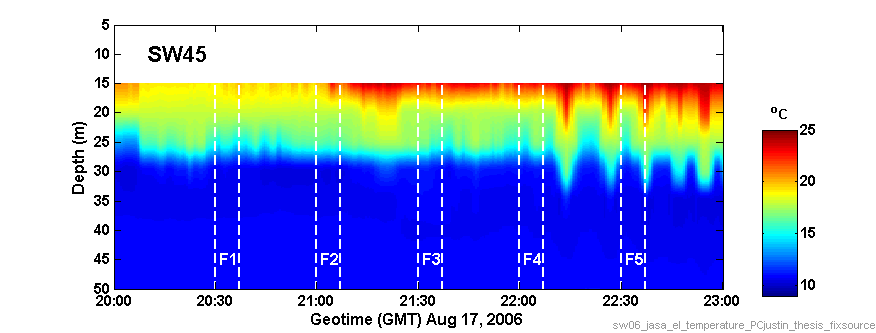
\includegraphics[width=0.8\textwidth]{jasa_el_sw45_fig1_thesis.png}
            \label{fig:sw45_fix}}
        \subfigure{
            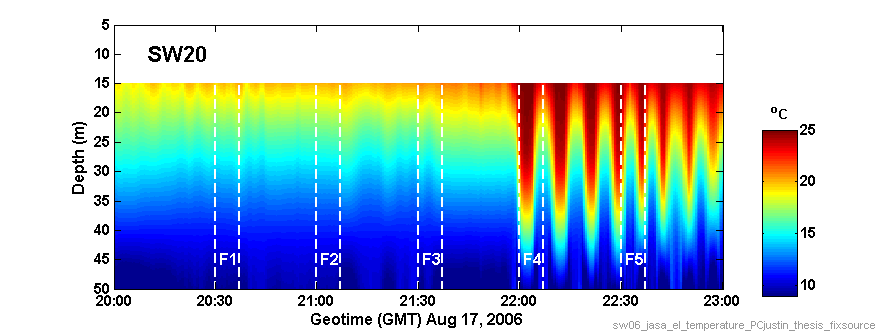
\includegraphics[width=0.8\textwidth]{jasa_el_sw20_fig1_thesis.png}
            \label{fig:sw20_fix}}
        \subfigure{
            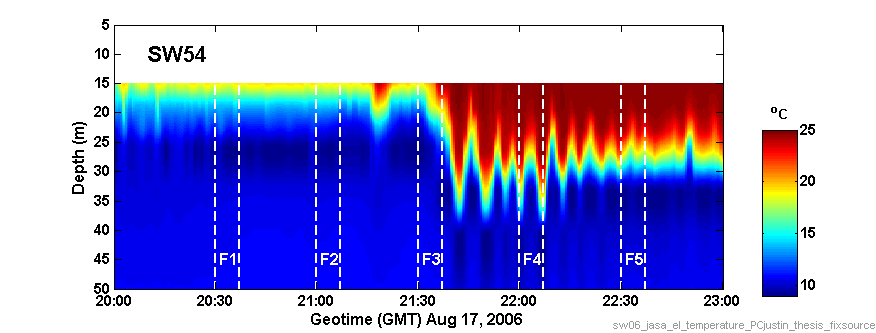
\includegraphics[width=0.8\textwidth]{jasa_el_sw54_fig1_thesis.png}
            \label{fig:sw54_fix}}
    \caption{Temperature record at three location along the fixed sourc-receiver track. Panel (a), (b) and (c) show the temperature at the NRL300 source (SW45), the midpoint (SW20) and the Shark VLA (SW54).}
    \label{fig:nrl300_temp_1}
\end{figure}

\begin{figure}[!ht]
        \subfigure{
        \centering
            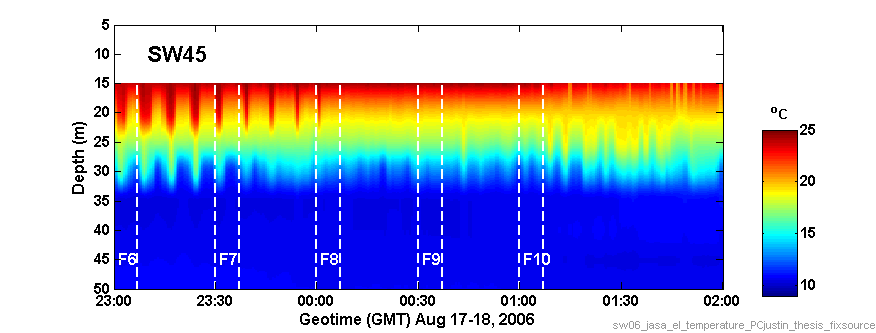
\includegraphics[width=0.8\textwidth]{jasa_el_sw45_fig2_thesis.png}
            \label{fig:sw45_fix}}
        \subfigure{
            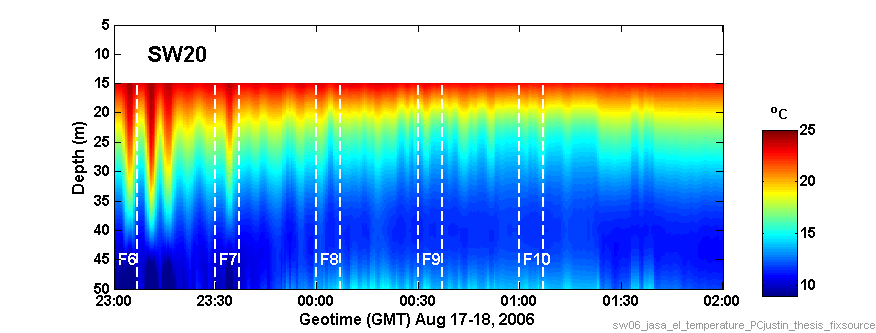
\includegraphics[width=0.8\textwidth]{jasa_el_sw20_fig2_thesis.png}
            \label{fig:sw20_fix}}
        \subfigure{
            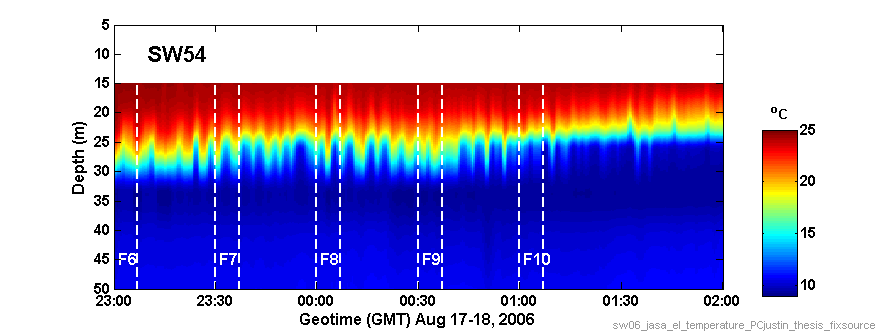
\includegraphics[width=0.8\textwidth]{jasa_el_sw54_fig2_thesis.png}
            \label{fig:sw54_fix}}
    \caption{Temperature record at three location along the fixed sourc-receiver track. Panel (a), (b) and (c) show the temperature at the NRL300 source (SW45), the midpoint (SW20) and the Shark VLA (SW54).}
    \label{fig:nrl300_temp_2}
\end{figure}
%
%\begin{figure}[H]
% \centering
% 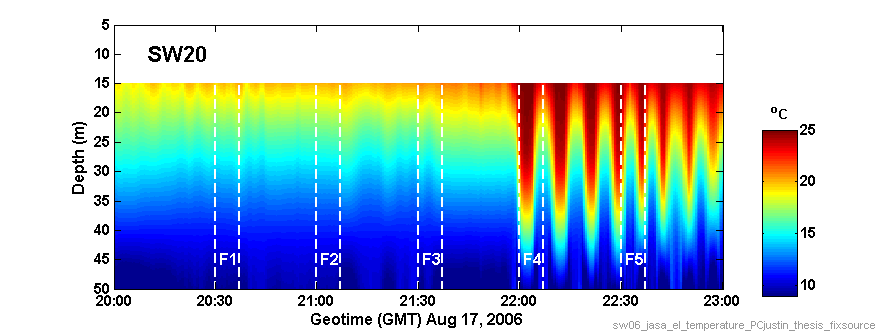
\includegraphics[width=0.5\textwidth]{jasa_el_sw20_fig1_thesis.png}
% \caption{Temperature record at three location along the fixed sourc-receiver track. Panel (a), (b) and (c) show the temperature at the NRL300 source (SW45), the midpoint (SW20) and the Shark VLA (SW54).}\label{fig:nrl300_temp}
%\end{figure}


\begin{figure}[H]
  \centering
  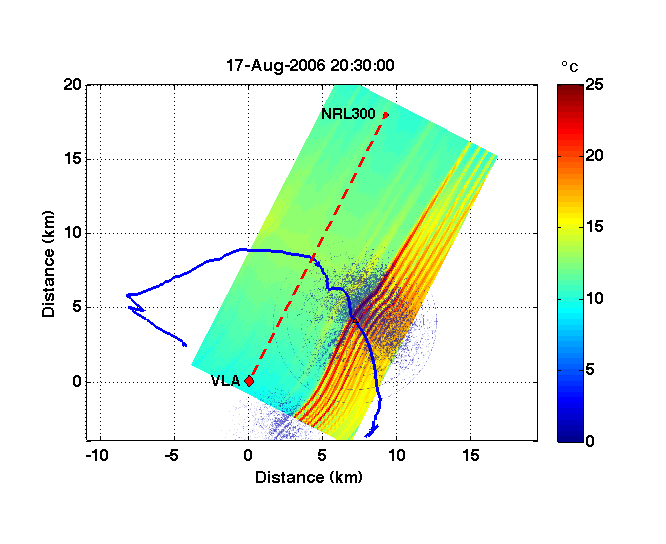
\includegraphics[width=\textwidth]{sw06_Tempr_Depth30m_2006Aug17_203000_radar_curve_thesis1.png}
  \caption{Interpolated internal wave field at 20:30GMT, Aug. 17, water depth = 20m. (Refer to section 3.4 for detailed interpolation method)}\label{fig:r2030_i}
\end{figure}

\begin{figure}[H]
  \centering
  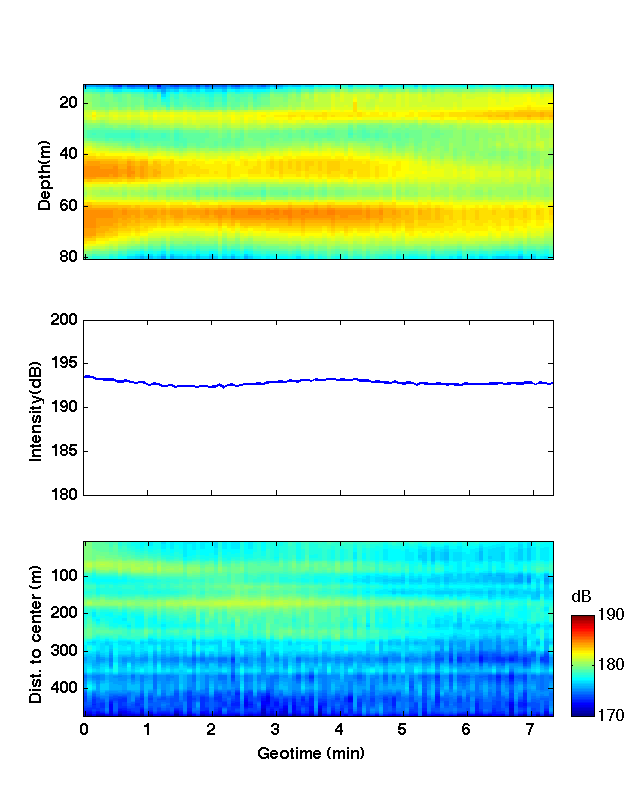
\includegraphics[width=\textwidth]{nrl300_060817T2030_vla_hla_intens_geotime2.png}
  \caption{Received signal on Shark VLA (top), HLA (bottom) and signal intensity (middle) from Aug.17 20:30GMT to 20:37GMT }\label{fig:a2030}
\end{figure}

\begin{figure}[H]
  \centering
  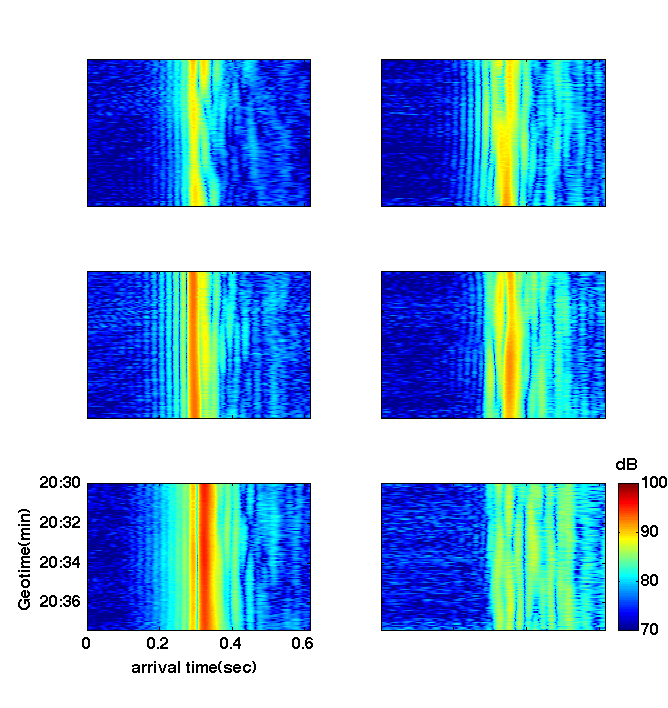
\includegraphics[width=\textwidth]{sw06_broadband_mf_nrl300_F1_6in1_thesis.png}
  \caption{Mode decomposition of received signal on Shark VLA. 
    Left column: mode 1-3, right column: mode 4-6 }\label{fig:m2030}
\end{figure}



%%--F2
\begin{figure}[H]
  \centering
  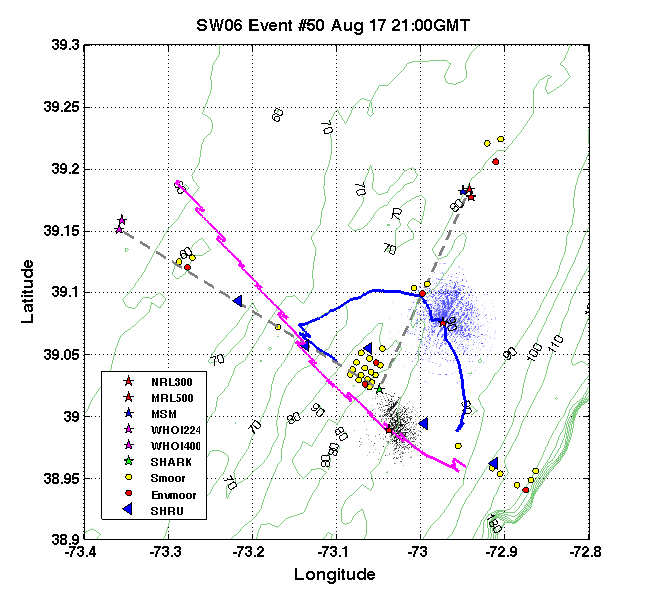
\includegraphics[width=\textwidth]{Aug17_2100_t.png}
  \caption{Surface expression of internal wave package at 21:00GMT, Aug. 17, recorded by R/V Sharp and R/V Oceanus. Blue and red lines indicate their movements, respectively. (Blue: R/V Sharp's, red: R/V Oceanus'}\label{fig:r2100_r}
\end{figure}

\begin{figure}[H]
  \centering
  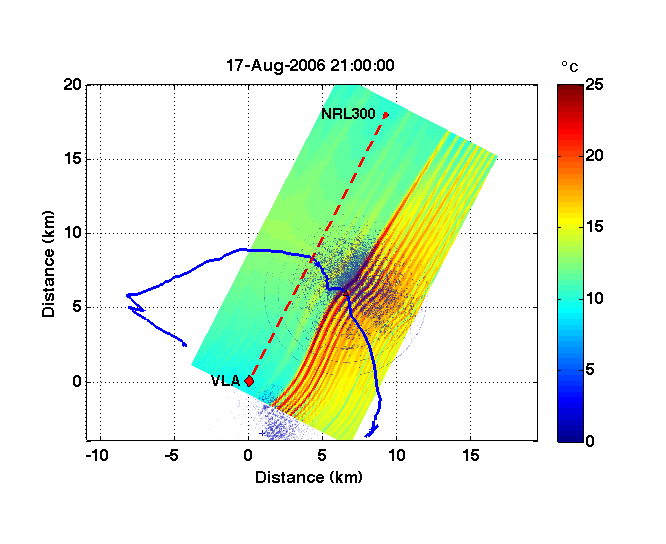
\includegraphics[width=\textwidth]{sw06_Tempr_Depth30m_2006Aug17_210000_radar_curve_thesis1.png}
  \caption{Interpolated internal wave field at 21:00GMT, Aug. 17, water depth = 20m. (Refer to section 3.4 for detailed interpolation method)}\label{fig:r2100_i}
\end{figure}

\begin{figure}[H]
  \centering
  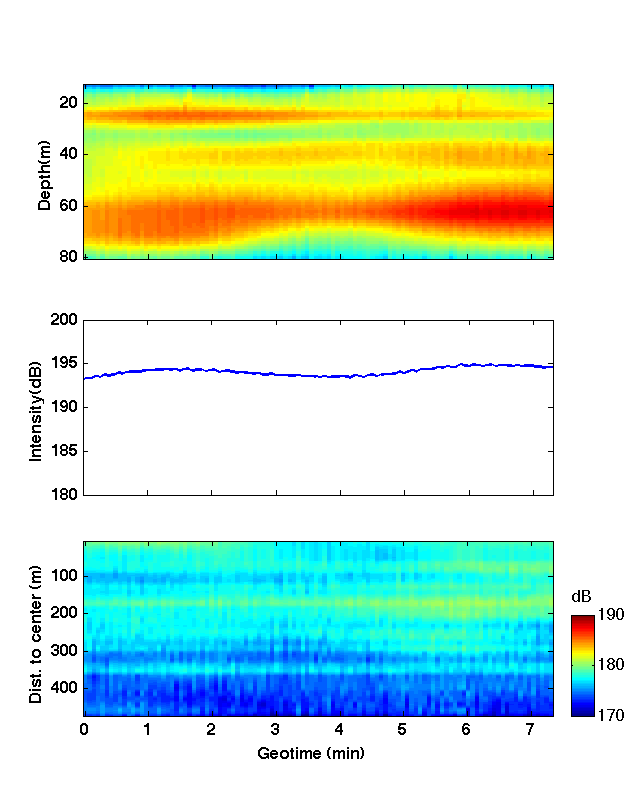
\includegraphics[width=\textwidth]{nrl300_060817T2100_vla_hla_intens_geotime2.png}
  \caption{Received signal on Shark VLA (top), HLA (bottom) and signal intensity (middle) from Aug.17 21:00GMT to 21:07GMT }\label{fig:a2100}
\end{figure}

\begin{figure}[H]
  \centering
  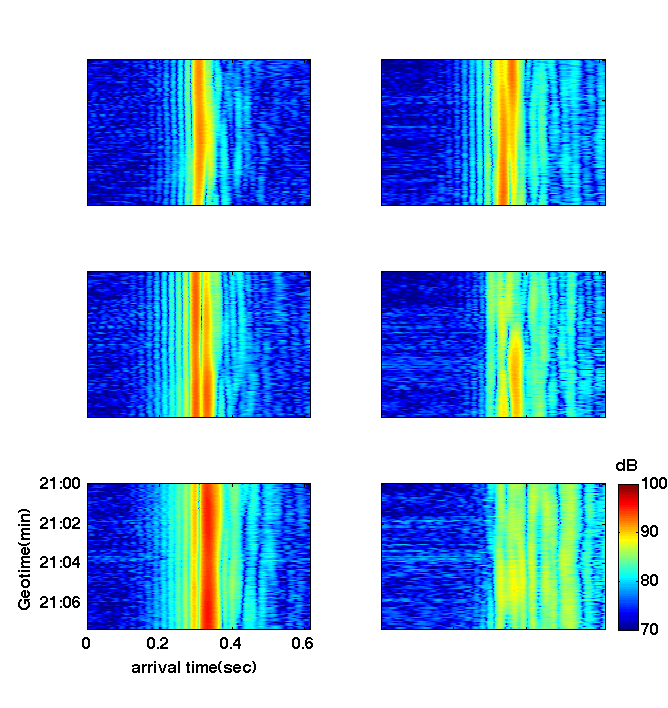
\includegraphics[width=\textwidth]{sw06_broadband_mf_nrl300_F2_6in1_thesis.png}
  \caption{Mode decomposition of received signal on Shark VLA. 
    Left column: mode 1-3, right column: mode 4-6 }\label{fig:m2100}
\end{figure}


\begin{figure}[H]
  \centering
  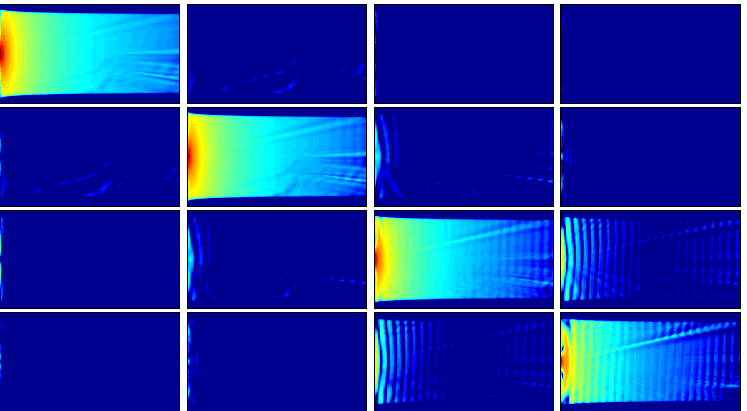
\includegraphics[width=\textwidth]{MC_17Aug06_210500_m_all.png}
  \caption{Mode coupling between mode 1~4 }\label{fig:mc2130}
\end{figure}


%--F3
\begin{figure}[H]
  \centering
  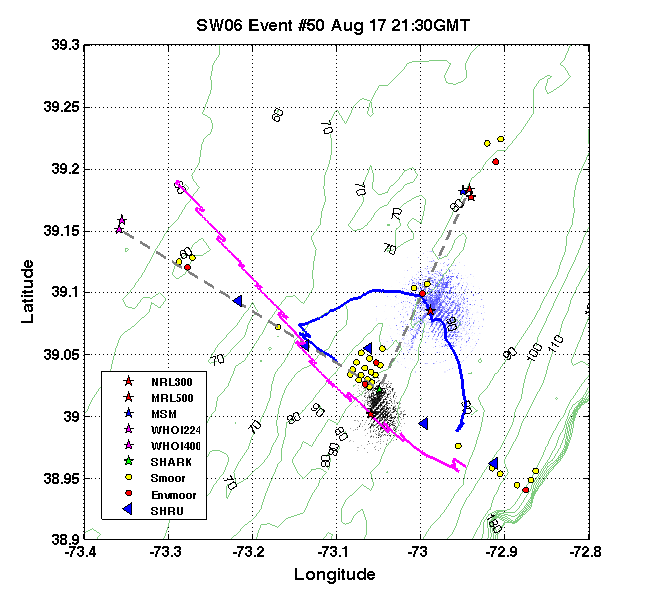
\includegraphics[width=\textwidth]{Aug17_2130_t.png}
  \caption{Surface expression of internal wave package at 21:30GMT, Aug. 17, recorded by R/V Sharp and R/V Oceanus. Blue and red lines indicate their movements, respectively. (Blue: R/V Sharp's, red: R/V Oceanus'}\label{fig:r2130_r}
\end{figure}

\begin{figure}[H]
  \centering
  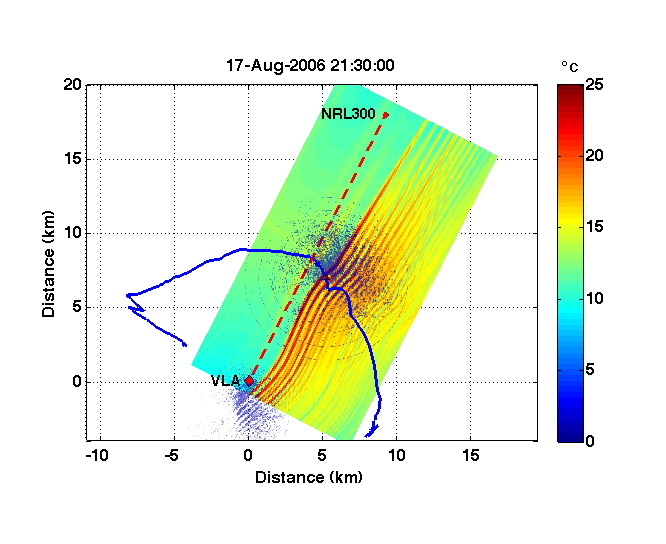
\includegraphics[width=\textwidth]{sw06_Tempr_Depth30m_2006Aug17_213000_radar_curve_thesis1.png}
  \caption{Interpolated internal wave field at 21:30GMT, Aug. 17, water depth = 20m. (Refer to section 3.4 for detailed interpolation method)}\label{fig:r2130_i}
\end{figure}

\begin{figure}[H]
  \centering
  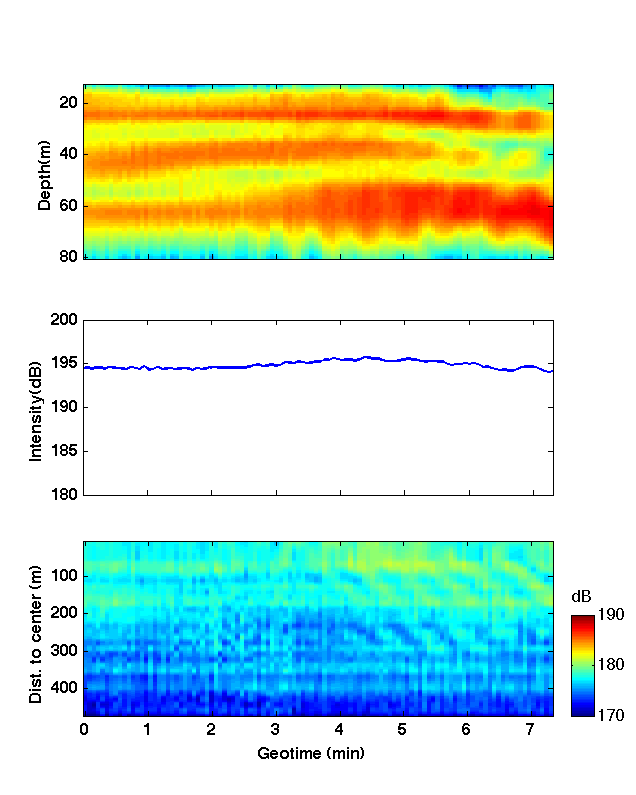
\includegraphics[width=\textwidth]{nrl300_060817T2130_vla_hla_intens_geotime2.png}
  \caption{Received signal on Shark VLA (top), HLA (bottom) and signal intensity (middle) from Aug.17 21:30GMT to 21:37GMT }\label{fig:a2130}
\end{figure}

\begin{figure}[H]
  \centering
  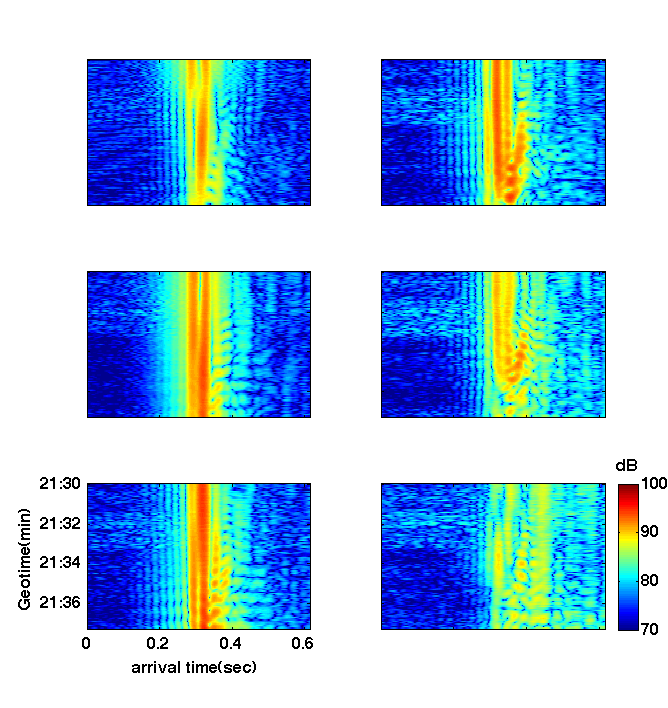
\includegraphics[width=\textwidth]{sw06_broadband_mf_nrl300_F3_6in1_thesis.png}
  \caption{Mode decomposition of received signal on Shark VLA. 
    Left column: mode 1-3, right column: mode 4-6 }\label{fig:m2130}
\end{figure}
\clearpage

%%--F4
\begin{figure}[H]
  \centering
  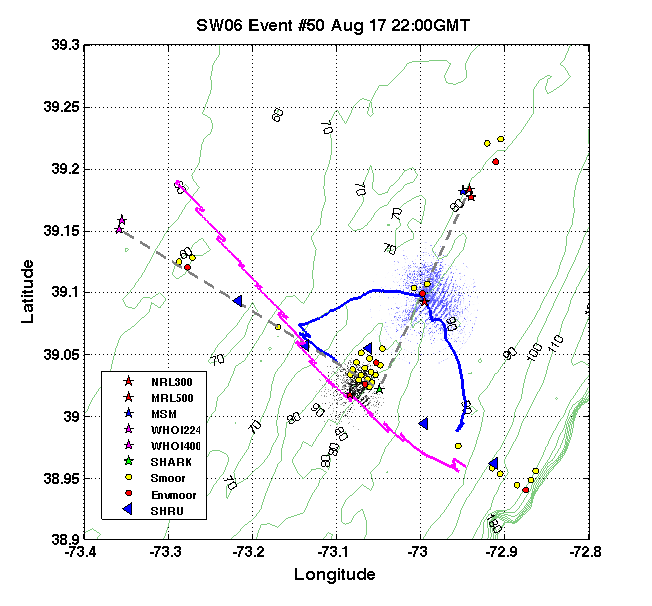
\includegraphics[width=\textwidth]{Aug17_2200_t.png}
  \caption{Surface expression of internal wave package at 22:00GMT, Aug. 17, recorded by R/V Sharp and R/V Oceanus. Blue and red lines indicate their movements, respectively. (Blue: R/V Sharp's, red: R/V Oceanus'}\label{fig:r2200_r}
\end{figure}

\begin{figure}[H]
  \centering
  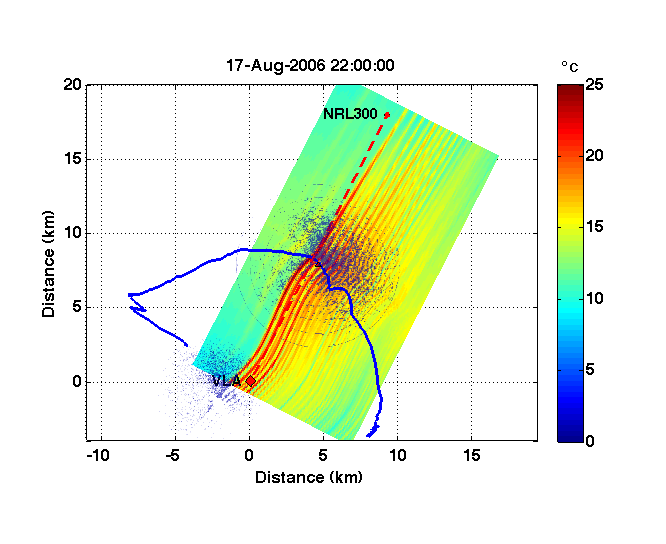
\includegraphics[width=\textwidth]{sw06_Tempr_Depth30m_2006Aug17_220000_radar_curve_thesis1.png}
  \caption{Interpolated internal wave field at 22:00GMT, Aug. 17, water depth = 20m. (Refer to section 3.4 for detailed interpolation method)}\label{fig:r2200_i}
\end{figure}

\begin{figure}[H]
  \centering
  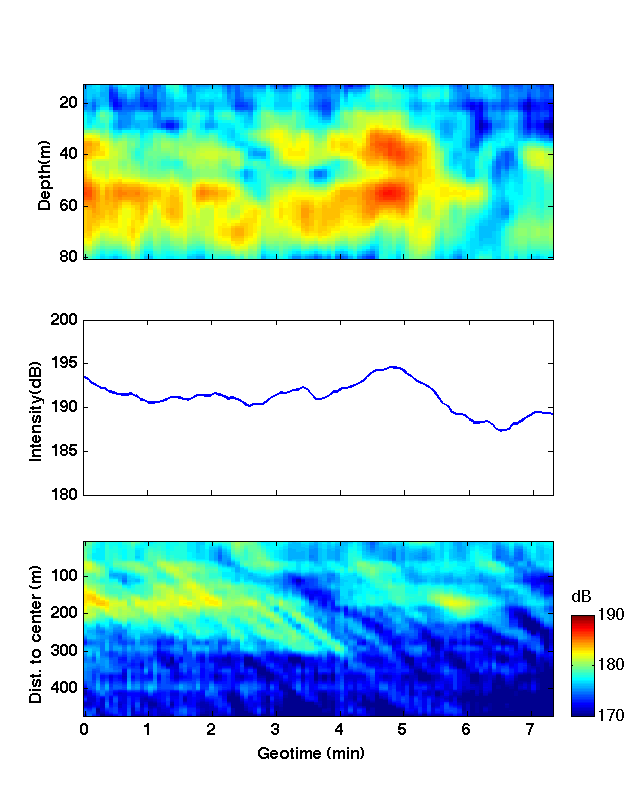
\includegraphics[width=\textwidth]{nrl300_060817T2200_vla_hla_intens_geotime2.png}
  \caption{Received signal on Shark VLA (top), HLA (bottom) and signal intensity (middle) from Aug.17 22:00GMT to 22:07GMT }\label{fig:a2200}
\end{figure}

\begin{figure}[H]
  \centering
  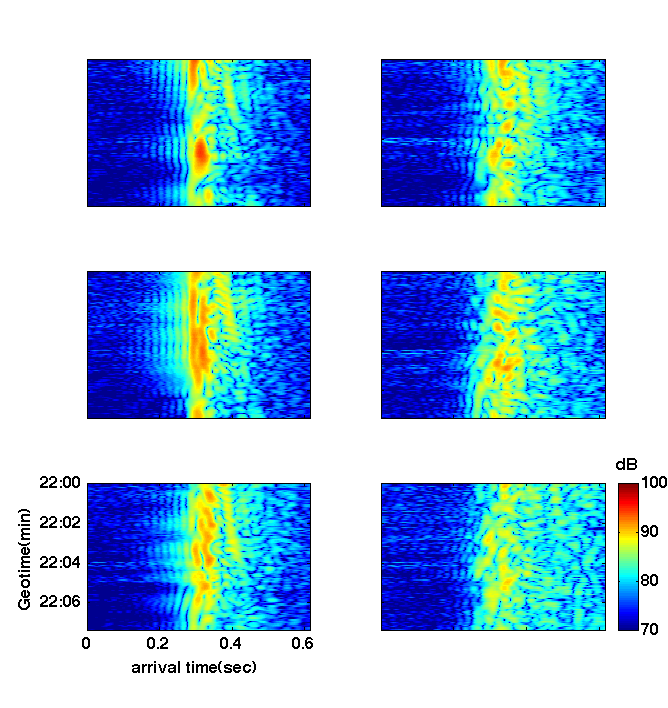
\includegraphics[width=\textwidth]{sw06_broadband_mf_nrl300_F4_6in1_thesis.png}
  \caption{Mode decomposition of received signal on Shark VLA. 
    Left column: mode 1-3, right column: mode 4-6 }\label{fig:m2200}
\end{figure}


%%--F5
\begin{figure}[H]
  \centering
  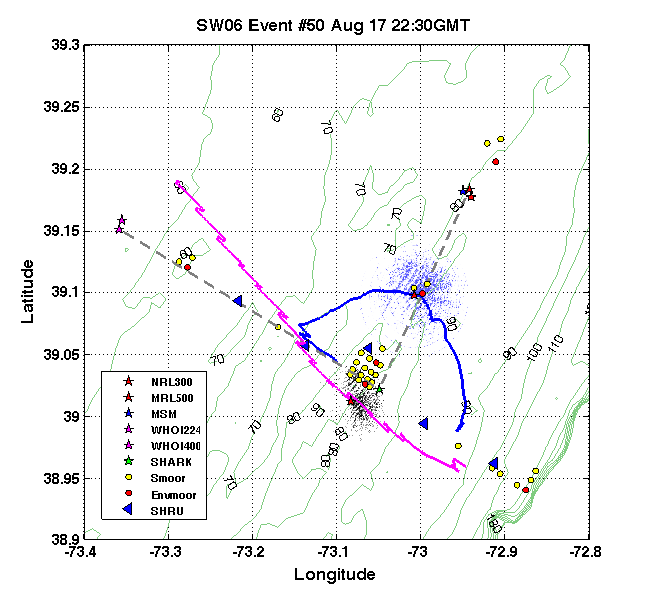
\includegraphics[width=\textwidth]{Aug17_2230_t.png}
  \caption{Surface expression of internal wave package at 22:30GMT, Aug. 17, recorded by R/V Sharp and R/V Oceanus. Blue and red lines indicate their movements, respectively. (Blue: R/V Sharp's, red: R/V Oceanus'}\label{fig:r2230_r}
\end{figure}

\begin{figure}[H]
 \centering
 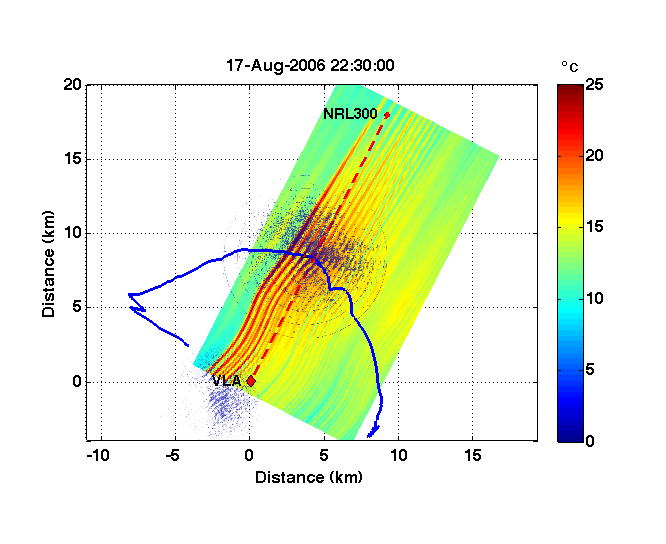
\includegraphics[width=\textwidth]{sw06_Tempr_Depth30m_2006Aug17_223000_radar_curve_thesis1.png}
 \caption{Interpolated internal wave field at 22:30GMT, Aug. 17, water depth = 20m. (Refer to section 3.4 for detailed interpolation method)}\label{fig:r2230_i}
\end{figure}

\begin{figure}[H]
  \centering
  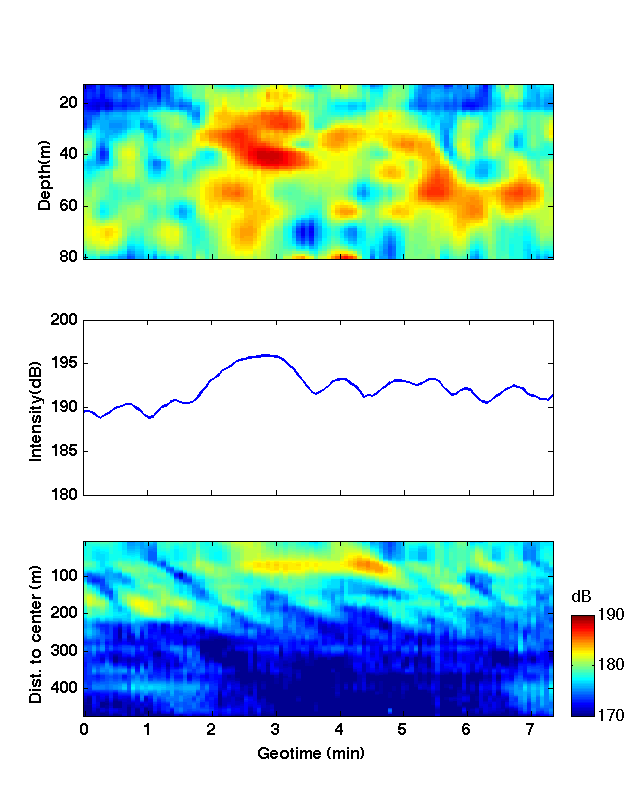
\includegraphics[width=\textwidth]{nrl300_060817T2230_vla_hla_intens_geotime2.png}
  \caption{Received signal on Shark VLA (top), HLA (bottom) and signal intensity (middle) from Aug.17 22:30GMT to 22:37GMT }\label{fig:a2230}
\end{figure}

\begin{figure}[h]
\centering
 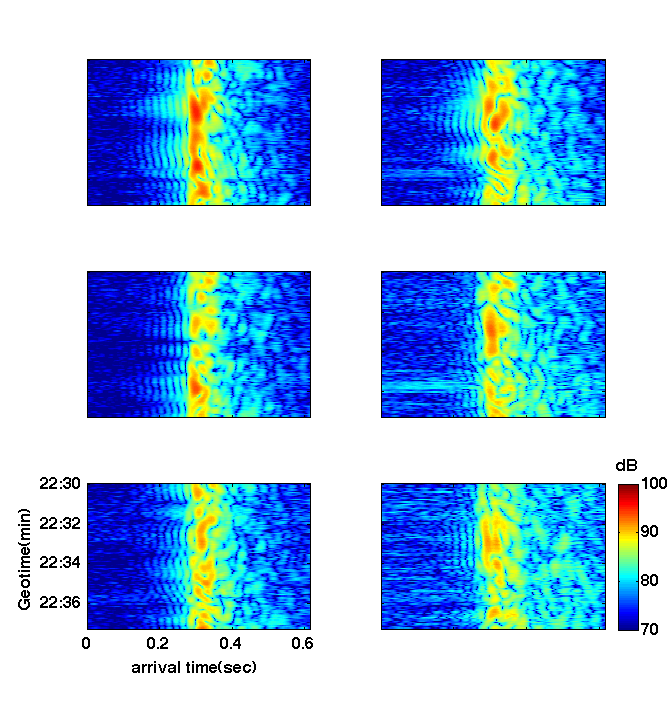
\includegraphics[width=\textwidth]{sw06_broadband_mf_nrl300_F5_6in1_thesis.png}
  \caption{Mode decomposition of received signal on Shark VLA. 
    Left column: mode 1-3, right column: mode 4-6 }\label{fig:m2230}
\end{figure}


